\documentclass[titlepage]{article}
\usepackage[utf8]{inputenc}
\usepackage{hyperref}
\usepackage{csquotes}
\usepackage{listings}
\usepackage{float}
\usepackage{graphicx}
\usepackage{comment}
\usepackage[
backend=biber,
style=alphabetic,
sorting=ynt]{biblatex}
 
\usepackage[nonumberlist,acronymlists={gloss}]{glossaries}
\makeglossaries

\newglossaryentry{latex}
{
	name=latex,
	description={A markup language}
}


\addbibresource{bibliography.bib}
\title{Doble factor de autenticación independiente de SO}
\author{Roselló Morell, Sergio\\
\texttt{sergio.rosello@live.u-tad.com}}

\begin{document}

\maketitle
\tableofcontents
\clearpage
\section{Agradecimientos}
Debo agradecer a Eduardo Ariols, mi tutor del trabajo todo el apoyo y consejos dados. Estoy seguro de que sin su ayuda, este trabajo no hubiese llegado a su nivel actual. Durante el proceso de elección del trabajo, me ayudó a darme cuenta de lo que quería hacer exactamente y desde ese momento, no ha parado de inspirarme con distintas formas de ver las cosas. De eso, le estoy muy agradecido.\\También quiero agradecer a la universidad el buen trabajo a la hora de escoger al personal docente de mi grado, puesto que en todo momento han demostrado más que profesionalidad y compañerismo hacia mi y mis compañeros de carrera.
\clearpage
\section{Resumen}
Este documento explica al lector la experiencia que he tenido durante el periodo de realización del trabajo de final de grado. Este trabajo trata sobre la autenticación de un usuario a un sistema \Gls{GNU/Linux}, en concreto, mediante una llave \Gls{USB}.\\Durante la fase de investigación de las tecnologías existentes, encontré algunas que ofrecían usa solución elegante, mediante \Gls{dbus} pero acabando la fase de investigación encontré un proyecto llamado \Gls{PAM} que redefinió la forma en la que planteaba el trabajo. Ésta es la forma por defecto de autenticar a los usuarios que tienen la mayoría de sistemas \Gls{GNU/Linux}.\\Este trabajo, al principio con enfoque mucho más práctico ha acabado teniendo un enfoque investigativo puesto que para implementar el módulo de autenticación, he tenido que construir una base fuerte sobre la que sentirme cómodo. Esta base es la que he tenido que esforzarme a entender puesto a que sin ella, el trabajo realizado, aunque funcionalmente completo, no me hubiese sido ni la mitad de estimulante e interesante.

\begin{abstract}
	This document reports my experience as I work on creating a USB-centric authentication method for \Gls{GNU/Linux}. During the research phase, I came across several elegant implementations, all of them worked with \Gls{dbus}. During the final stages of this period, I discovered \Gls{PAM} which changed my whole perspective on this project. Most of \Gls{GNU/Linux} systems use this module to enable authentication for their users.\\At the start of this project I would've expected to code a lot more, but now I realise that without a solid foundation, I may have been able to do what I had proposed, but I would not have the understanding on how the \Gls{PAM} fits into the whole equation and the many benefits it provides. This, I think is the point of this work.
\end{abstract}
\clearpage
\printglossary[title={Abreviaciones y tecnicismos}]
\clearpage
\begin{comment}
	hola
\section{Motivación}
Durante el transcurso del grado me he visto cada vez más interesado en la arquitectura \Gls{GNU/Linux}. A pesar de que no he impartido asignaturas orientadas a estos sistemas, mi propio interés y la base proporcionada por la carrera me han incitado a entrar en el mundo de GNU/Linux. Durante el transcurso de la carrera, he pasado de Ubuntu hasta Arch, profundizando poco a poco en el funcionamiento de estos sistemas GNU/Linux. Este trabajo representa la comprensión y desempeño que he adquirido a lo largo de la carrera.\\Lo que quiero conseguir es implementar un \Gls{DFA} en mi ordenador de forma que pueda bloquearlo si extraigo un USB específico. Una vez conseguido esto, haré la operación inversa. Conseguir desbloquear mi ordenador insertando un USB específico.\\Para finalizar, proporcionar una interfaz para decidir que quiere habilitar o deshabilitar el usuario del programa. La herramienta en la que me voy a enfocar para hacer esto bien va a ser dbus, una aplicación que crea un protocolo de comunicación que pueden usar los programas del ordenador para comunicarse entre ellos.\\Durante el desarrollo del trabajo he descubierto un módulo llamado \textit{\Gls{PAM}}. Este módulo ofrece a los administradores de sistemas una forma centralizada de autenticación que pueden usar la gran mayoría de aplicaciones. Ofrece también a los desarrolladores control y flexibilidad sin tener que esforzarse en implementar un esquema de autenticación y simplemente centrarse en su proyecto.
\section{Estado del arte}
He encontrado varios métodos de desbloquear/bloquear el ordenador, los he catalogado en Hardware y Software.
\subsection{Hardware}
Estos dispositivos sirven para asegurar que el usuario es realmente quien tiene que ser. Existen varias marcas que ofrecen el mismo servicio, pero \href{https://www.yubico.com/why-yubico/for-individuals/}{yubico} es la original.
Esta llave USB integra varias tecnologías. Existe la opción de usar un \textit{\Gls{OTP}}, \textit{\Gls{OATH}}, \textit{\Gls{OpenPGP}} y otras tecnologías de inicio de sesión.

\subsection{software}
Para buscar proyectos parecidos a lo que quiero hacer, he buscado en \href{https://github.com/}{GitHub}. Muchos de los proyectos no cumplen con las especificaciones que quiero implementar en mi proyecto. 
\subsubsection{Usblock \cite{usblock}}
Este proyecto consigue lo que yo quiero hacer, el problema es que no ha sido actualizado y por tanto ha quedado deprecado. El hecho de que use la capa \textit{\Gls{HAL}} hace que la mayoría de sistemas nuevos, por no decir todos van a ser incompatibles con este programa. Esta capa ha sido reemplazada por \Gls{udev} \cite{udev}.
\subsubsection{\textit{\Gls{PAM}}}
Este proyecto es un adaptador entre los nuevos protocolos de inicio de sesión y los programas que los utilizan. De esta forma, el desarrollador del programa no tiene que actualizar el software que ya ha escrito para dar soporte al nuevo método de autenticación, simplemente implementa \textit{\Gls{PAM}}. La \href{http://www.linux-pam.org/Linux-PAM-html/}{documentación} incluye guías para administradores de sistemas y programadores.
\section{Propuesta}
Los proyectos vistos anteriormente, aunque interesantes, no cumplen con todas las características que quiero integrar en mi proyecto.\\Metas:
\begin{itemize}
	\item Inicio de sesión con USB al sistema
	\item Inicio de sesión con USB y contraseña al sistema (Doble factor de autenticación)
	\item Interfaz centralizada que gestione y facilite la tarea al usuario
	\item Ampliar la herramienta para que integre múltiples formas de autenticar al usuario
\end{itemize}
\section{Investigación inicial para realizar la herramienta}
Los sistemas \Gls{GNU/Linux} tienen un gestor de contraseñas llamado \textit{\Gls{PAM}}. Este gestor unifica las distintas formas de autenticar a un usuario en un sistema o aplicación. La mayor parte de sistemas/aplicaciones usan este módulo para autenticar a sus usuarios. Existe también un módulo que integra el motor \textit{\Gls{PAM}} para autenticar mediante USB a los usuarios. Se llama \textit{\Gls{PAMUSB}}. Es un módulo bastante extendido y usado, además la \href{http://www.pamusb.org/#hotplug}{documentación} es buena.
\section{Puesta a punto}
Para hacer este proyecto, necesito una serie de programas/demonios sobre los que poder trabajar. A continuación explico porque y como llego a elegir los que uso. 
\subsection{Dependencias básicas}
Para iniciar el proyecto, asumo que no tenemos nada de lo que necesitamos para llevarlo a cabo, aunque la mayoría de distribuciones de \Gls{GNU/Linux} vienen con un gestor de USB ya preinstalado, no debemos obviarlo como dependencia del proyecto ya que aunque insertemos el USB en la ranura USB de nuestro ordenador, si no lo montamos en nuestro sistema, no va a aparecer disponible en nuestro módulo \textit{\Gls{PAMUSB}}.
\subsubsection{UDisks}
Dado que una de las dependencias básicas del proyecto es un gestor de USBs para montar el almacenamiento en el sistema, procedo a investigar el gestor más adecuado para el proyecto. Para facilitar la tarea de montar el USB en el sistema, usamos \textit{\Gls{udevil}} \cite{udevil}
\end{comment}
\section{Estado del arte}
La forma en la que se autentica la identidad de los usuarios de sistemas ha ido evolucionando desde que se vio que era necesaria.
\subsection{Inicios de la gestión de permisos}
Cada objeto tiene asociada una tabla de 9 bits, los tres primeros indican los privilegios de lectura, escritura y ejecución del usuario que posee el objeto. Los tres siguientes son para la lectura, escritura y ejecución de los usuarios pertenecientes al grupo que posee el objeto y los tres últimos son de lectura, escritura y ejecución de los usuarios que no pertenecen a ninguno de las dos primeras categorías. Esta categoría se llama \textit{others}. Además de estos 9 bits, también pueden incluir el \Gls{SetUid}, \Gls{SetGid} y el \Gls{StickyBit}. A pesar de ser un sistema muy simple de gestionar privilegios, cumple la mayoría de escenarios posibles en sistemas UNIX e incluso a día de hoy, se sigue usando en todos los sistemas \Gls{GNU/Linux} ya que proporciona una forma sencilla y eficiente de visualizar los privilegios de los objetos y modificarlos. Esta forma de gestionar los privilegios de los objetos se puede denominar \Gls{ACL}.
\begin{figure}[H]
    \centering
    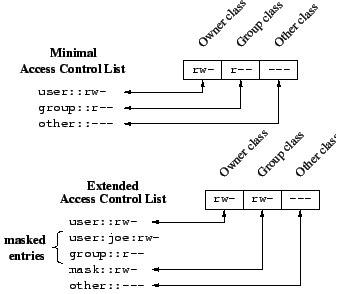
\includegraphics[width=0.5\textwidth]{Media/ACL.jpg}
    \caption{\Gls{ACL}}
    \label{fig:ACL}
\end{figure}
\subsection{\Gls{RBAC}}
Este esquema de seguridad está diseñado para organizaciones o sistemas en los que van a interactuar distintos usuarios con una gran cantidad de datos. El sistema defiende que, en lugar de tener una tabla por cada objeto, definiendo la forma que tienen los usuarios de interactuar con él, se deberían establecer una serie de transacciones, que dependiendo del rol serán distintas. Estas transacciones, una vez definidas cambian poco porque un usuario específico va a usar unos documentos específicos, dependiendo de la responsabilidad que tenga en la organización. En la imagen \ref{fig:RBAC} se puede ver claramente como dependiendo del rol vas a poder acceder a ciertos objetos.
\begin{figure}[H]
    \centering
    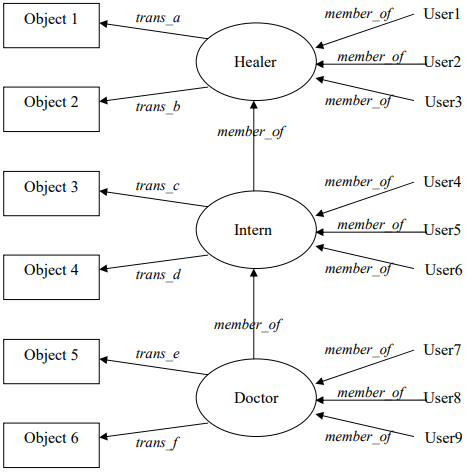
\includegraphics[width=0.5\textwidth]{Media/RBAC.PNG}
    \caption{\Gls{RBAC}}
    \label{fig:RBAC}
\end{figure}
Dos de las ventajas de este sistema son que cumplir el principio de de menor privilegio es relativamente sencillo, ya que se puede conseguir no proporcionándole  al usuario más transacciones de las que debe tener. Otra de las ventajas, innata, de \Gls{RBAC} es la separación de deberes. Esto es: En el caso de tener que realizar un transferencia bancaria, nunca se debería de poder proporcionar al mismo individuo el control de todo el flujo, ya que se le está dando la oportunidad de cometer algún tipo de irregularidad. Con RBAC puedes asignar dos transacciones, una que permita a un usuario solicitar una transferencia y otra que permita a un usuario validar la transferencia.
\subsection{\Gls{PAM}}

\clearpage
\printbibliography[heading=bibintoc,title={Bibliografía}]
\end{document}

